\section{Simulating and recording scientific data}\label{sec:mat}
History about synthesis, screening, characterization, discovery and re-discovery (retrieval)

%Table with all the image modalities discussed in this paper

% Please add the following required packages to your document preamble:
% \usepackage[table,xcdraw]{xcolor}
% If you use beamer only pass "xcolor=table" option, i.e. \documentclass[xcolor=table]{beamer}
\begin{table*}[!]
\centering
\caption{Scientific data under scrutiny with CNN: specifications and methods}
\label{table1}
\begin{tabular}{p{2cm}p{1.6cm}p{1.6cm}p{3cm}p{7.5cm}}
\hline
\rowcolor[HTML]{CCE5FF}
Materials  &  Resolution ($\mu$m)  &  Image \newline modality  &  Imaging  \newline mechanism  &  Data analysis for specimen quantification
\\
\hline
\rowcolor[HTML]{FFFFFF}
material2 \newline whatever & 0.65 to 1.3 & microCT                               & cryo-EM                     & detection something with MatConvNet. Sec.~\ref{subsec:cmc}. Fig.~\ref{fig:microct}.
\\
\hline
\rowcolor[HTML]{F6F6F6}
bragg peaks of what? & 0.65 to 2.5  & diffraction pattern & X-ray diffraction  & detection of Bragg peaks from whatever specimens using MatConvNet. Sec.~\ref{subsec:cmc}. Fig.~\ref{fig:pmrf}.
\\
\hline
\rowcolor[HTML]{FFFFFF}
material2 \newline whatever & 0.65 to 1.3 & microCT  & X-ray attenuation contrast & detection of fiber profile, TensorFlow. Sec.~\ref{subsec:cmc}. Fig.~\ref{fig:microct}.
\\
\hline
\rowcolor[HTML]{F6F6F6}
thin films   & 0.00164  & STEM \newline tomography  & electron transmission    & pore organization across film, associated to level of pore coalescence; surface density analysis correlated to dielectric constant measurements. Sec.~\ref{subsec:stem}. Fig.~\ref{fig:stem}.
\\
\hline
\end{tabular}
\end{table*}


%------------------------------------------------------------------------------
%no worries, these marks will be eliminated
-------------------------------------------------------
\subsection{Cryo-EM}\label{subsec:cryo}
Why Cryo-EM?

An important protein is the Transcription initiation factor II because it makes up everything... It has been studied using .... Cryo-EM is a good deal because...

It's hard to get labelled cryo-EM because..., therefore we resort to simulation code to investigate polypeptides. The name of the code and the reference

The data consists of 64 by 64 projection images of TFIID along 9 viewing angles with random perturbation, noise free... What does it have to do with Figure~\ref{fig:cryo1}? What about Figure~\ref{fig:cryo2}?

9 views (evenly spaced on a sphere)
1000 simulated projection images
Projection Euler angles:

chosen randomly from 1 to 9,  generated randomly (uniform distribution) with


\begin{figure*}[!t]
\centering
\subfloat[Experimental molecule projections]{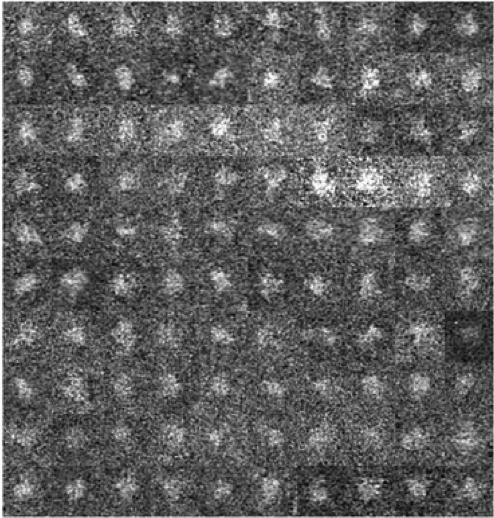
\includegraphics[width=.314\linewidth]{img/cryoem3a.png}
\label{fig_first_case}}
\hfil
\subfloat[Detected particle projections]{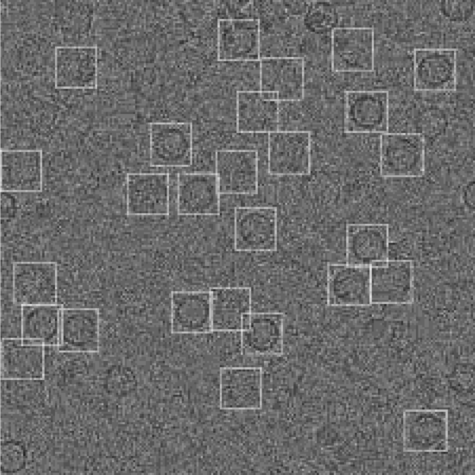
\includegraphics[width=.33\linewidth]{img/cryoem3b.png}
\label{fig_second_case}}
\subfloat[Simulated molecule projections]{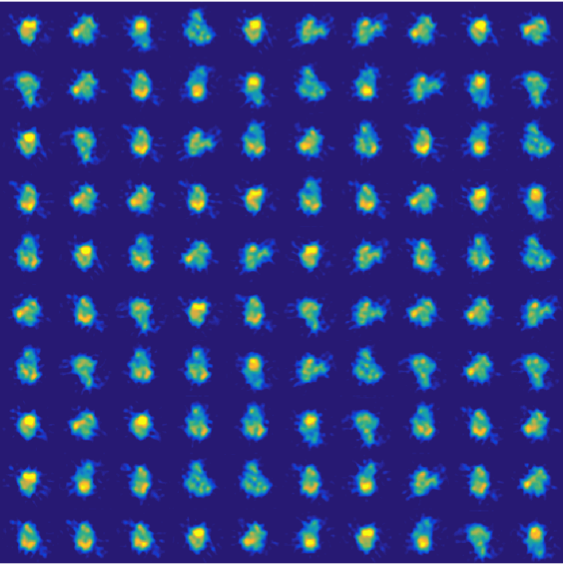
\includegraphics[width=.33\linewidth]{img/cryoem3c.png}
\label{fig_second_case}}
\caption{Cryo-EM images of TFIIDM at different project angles.}
\label{fig:cryo1}
\end{figure*}

\begin{figure*}[!t]
\centering
\subfloat[TFIIDM molecule]{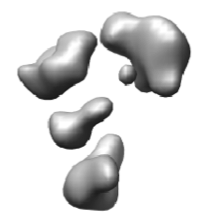
\includegraphics[width=.32\linewidth]{img/cryoem1.png}
\label{fig_first_case}}
\hfil
\subfloat[Projections model]{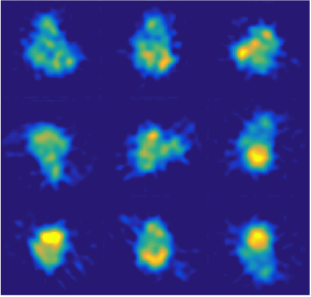
\includegraphics[width=.32\linewidth]{img/cryoem1b.png}
\label{fig_second_case}}
\subfloat[Compact model]{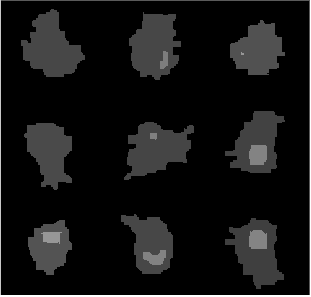
\includegraphics[width=.32\linewidth]{img/cryoem1c.png}
\label{fig_second_case}}
\caption{TFIIDM structure, cryo-EM simulation outcomes and reduced data representation.}
\label{fig:cryo2}
\end{figure*}

%------------------------------------------------------------------------------
%------------------------------------------------------------------------------
-------------------------------------------------------
\subsection{Imaging Techniques based on X-ray}


Synchrotron radiation relies on a charge moving at relativistic speeds, and following a curved trajectory~\cite{url:als:booklet}. The x-ray experimental data used in this article was acquired at the Advanced Light Source, which is a Department of Energy-funded synchrotron facility that provides users from around the world access to the brightest beams of soft x-rays, together with hard x-ray and infrared light, for scientific research and technology development in a wide range of disciplines~\cite{url:als}.

\subsubsection{X-ray diffraction}\label{subsec:diffraction} %LDRD Bragg peaks/Chao
92\% success rate for good images
96\% success rate for bad images
Sufficiently good to distinguish good images from bad images
%92% success rate on images with Bragg peaks
%96% success rate on images with few Bragg peaks

\begin{figure}[!t]
\centering
\subfloat[Hit]{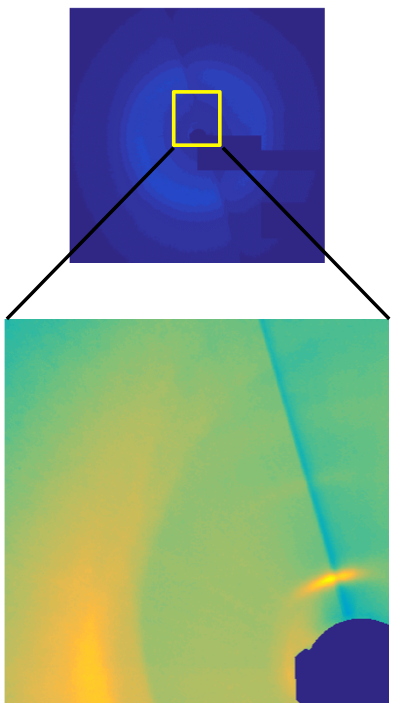
\includegraphics[width=.33\linewidth]{img/bragg1.png}
\label{fig_first_case}}
\hfil
\subfloat[Miss]{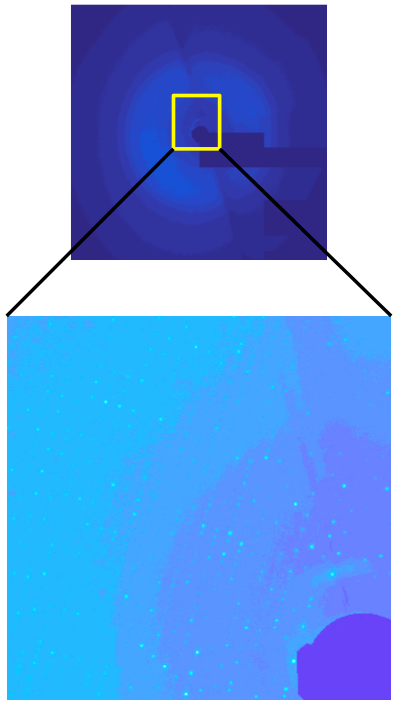
\includegraphics[width=.33\linewidth]{img/bragg2.png}
\label{fig_second_case}}
\caption{LDRD case - bragg peaks.}
\label{fig:ldrd}
\end{figure}

\begin{figure}[!t]
\centering
\subfloat[False negative]{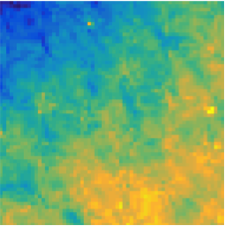
\includegraphics[width=.33\linewidth]{img/xdiffraction_falsenegative.png}
\label{fig_first_case}}
\hfil
\subfloat[False positive]{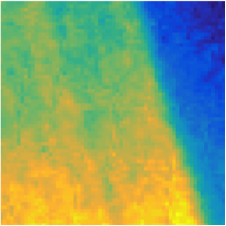
\includegraphics[width=.33\linewidth]{img/xdiffraction_falsepositive.png}
\label{fig_second_case}}
\caption{LDRD case - bragg peaks.}
\label{fig:ldrd}
\end{figure}

%------------------------------------------------------------------------------
-------------------------------------------------------
\subsubsection{X-ray scattering}\label{subsec:gisaxs} %Alex
Scattering techniques are very well established and used to probe micro and nano-structures with a high degree of statistical relevance. The most prominent techniques are small angle X-ray and neutron scattering (SAXS and SANS) for the detection of mesoscale structures as well as wide angle X-ray and neutron scattering (WAXS and WANS) for the investigation of the structure down to the molecular scale. Prominent examples are thin films of conductive polymers, organic electronics, or thin films of nano-particles, which receive high interest for energy relevant materials such as organic photovoltaics. Morphological characterization of thin films is challenging, and substantial advancements have been accomplished through research efforts on new experimental geometry setups for scattering. Unfortunately, these have not been enough to provide the required data reduction and analysis that is fundamental for giving scientist access to use advanced grazing incidence techniques and getting the most relevant information out of their experiments. In particular in-situ analysis is far from possible at the given time.

We propose a supervised classification approach to identify the crystal lattice types from a Grazing Incidence Small Angle X-ray Scattering (GISAXS) image. GISAXS is an important reciprocal-space imaging modality which provides statistical information about a sample in 3-D. GISAXS is widely used for
studying thin films that play a vital role as building blocks for the next generation of renewable energy technology. One challenge in GISAXS imaging is to accurately infer the crystal lattice corresponding to the sample from a single 2-D diffraction/scatter pattern.

\begin{figure}[!t]
\centering
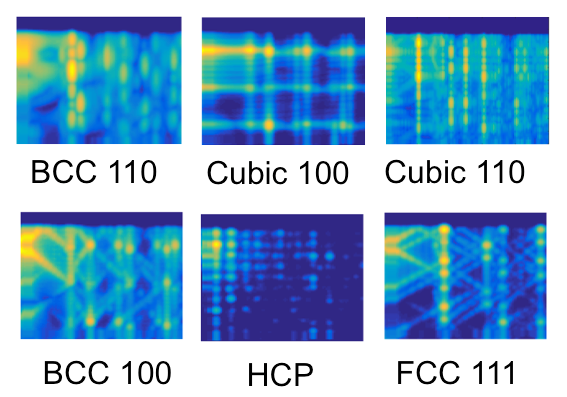
\includegraphics[width=.439\linewidth]{img/gisaxs1.png}
\caption{Figure to be replaced by Venkat.}
\label{fig:gisaxs}
\end{figure}

As a first step towards understanding crystal configurations, we use a simulation package termed HiPGISAXS [1], to generate a large collection of sample images from each class of possible crystal structures and test the algorithm performance under multiple simulated test images. Inspired by the
recent successes of deep-learning approaches for natural image classification, we tested CNN as the method to carry out the classification.

We have been exploring detection of peak-positions from image datasets, so that information about the lattice and orientation of the material is recovered. A typical image from the ALS beamline 7.3.3 will present shapes used as input to derive the underlying structure of the sample. The location, shapes and position of these structures, while yielding useful information, can also be used as an input to simulation tools. Shapes vary among rings, arcs, peaks and lines. In case of time resolved or multi-energy data, the features become three or more dimensional, e.g., peaks become rods and lines become planes. We will develop software tools for the pattern recognition of the scattering data collected in grazing incidence geometry. The task of extracting morphological structures and representing them through features maps will have similarities to pattern recognition in 3D tomography data. Advanced recognition will significantly accelerate the model development for forward solvers.

%------------------------------------------------------------------------------
-------------------------------------------------------
\subsubsection{X-ray attenuation contrast}\label{subsec:microct}
Another example of high-throughput data collection is microct....


the study of ceramic matrix composites, which are hierarchical materials, composed of many individual strands, bundled within a matrix, after which bundles are woven together. To simulate the operating conditions for which these materials are designed, they are heated to nearly 2,000 degrees and then stressed, causing both cracks in the matrix and the breaking of individual fibers. In both of the cases mentioned above, currently the researchers collect a series of 3D images as a function of time. After the experiment, the researchers often go through the 3D images manually, slice by slice, looking for the individual dendrites or “delaminations” that form in the batteries which correlate with decreased performance, or for the broken fibers or matrix cracks. This is a very time-consuming process.

Proposed work and expected solutions: Develop and deploy algorithms that find these features using raw microCT images as input, and then point out which of the experimental instances (image stacks) present the structures of interest. Being able to detect these features in real time will add an entirely new level of experimental capability. Tying this capability in with the control systems at the beamline will allow the experiment to be controlled by the machine in response to which structures the sample presents. For example, when a feature of interest is found, the process may be temporarily slowed down while a magnified image is collected of the region of interest, before resuming the process. Currently, it is unlikely that the users will find detailed features of interest in their images fast enough to be able to adjust the parameters of their experiment to collect optimal data. By having recognition closer to the detector, we will be able to obtain higher resolution data in specific regions, or more time points during a transition of interest.


\cite{IEEEBigData:2014}


\begin{figure}[!t]
\centering
\subfloat[Case I]{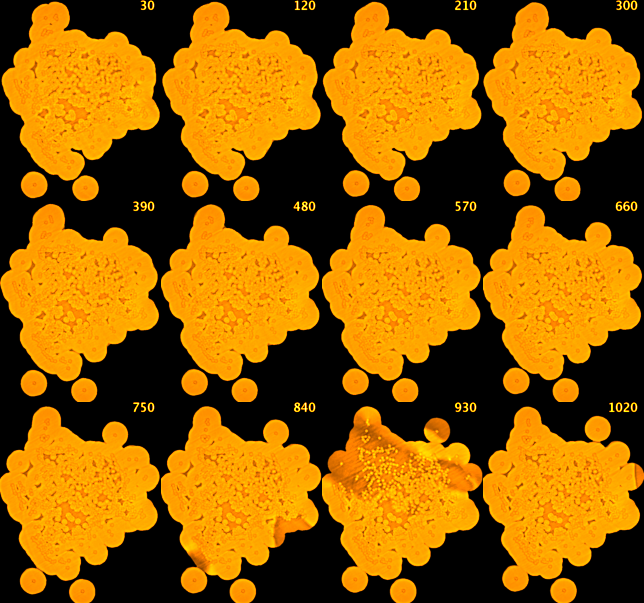
\includegraphics[width=.439\linewidth]{img/fiberMontage.png}
\label{fig_first_case}}
%\hfil
\subfloat[Case II]{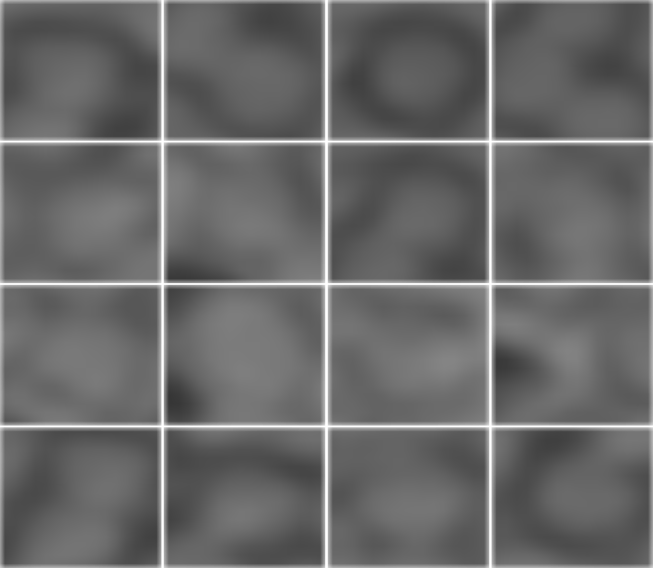
\includegraphics[width=.475\linewidth]{img/yes_fibers.png}
\label{fig_second_case}}
\caption{Some description of CMC and fibers.}
\label{fig:microct}
\end{figure}
